% TODO fill in your paper title
\newcommand{\PaperTitle}{Network Systems \& Design COLL 400 Capstone Project}
% TODO fill in your paper number when you get it
\newcommand{\PaperNumber}{XXX}

\documentclass[10pt,sigconf,letterpaper,nonacm]{acmart}

%%%%%%%%%%%%%%%%%%%%%%%%%%%%%%%%%%%%%%%%%%%%%%%%%%%%%%%%%%%%%%%%%%%%%%%%%%%%
% This is the preamble; include packages as you see fit.
% Here are a few recommendations:
% \usepackage{color}
% \usepackage{graphicx}
% \usepackage[labelformat=simple]{subcaption}
% \usepackage{xspace}
% \usepackage{multirow}
% \usepackage[ruled,vlined]{algorithm2e}
% \usepackage{ulem}
% \normalem

%%%%%%%%%%%%%%%%%%%%%%%%%%%%%%%%%%%%%%%%%%%%%%%%%%%%%%%%%%%%%%%%%%%%%%%%%%%%

\begin{document}

\title{\PaperTitle}

\author{Adam Chisholm}
\email{alchisholm@wm.edu}
\author{Conner Wright}
\email{cjwright03@wm.edu}
\author{Elijah Gilliam}
\email{kmgilliam@wm.edu}
\author{Zachary Klein}
\email{zaklein@wm.edu}
\affiliation{
  \institution{William \& Mary}
  \city{Williamsburg}
  \state{Virginia}
  \country{USA}
}

\begin{abstract}
    This project addresses the task of monitoring and classifying
network traffic by its originating website, with the goal of
enhancing network management, security, and performance
optimization. We collected a dataset of traffic records from
five popular websites: GitHub, Backloggd, Instagram, Letterboxd,
and Weather, and employed three machine learning models
for classification: Linear Regression, Logistic Regression, and
Random Forest. Comprehensive evaluation showed that the
Random Forest model achieved the highest accuracy (X)
and Macro F1 score (X), demonstrating its ability to handle
complex relationships within the dataset. The project
contributes to the field of network traffic classification by
demonstrating the feasibility of integrating machine learning
models into network traffic analysis, highlighting the
importance of dataset diversity, and providing a road-map
for future developments.
\end{abstract}

\keywords{Network Traffic Classification, Machine Learning, Classification Models}

\maketitle

\section{Introduction}
    Monitoring and classifying network traffic are critical tasks
for maintaining efficient network management, security, and
performance optimization [7]. The proliferation of diverse
online services necessitates robust methods to categorize
traffic patterns and accurately identify their sources [2]. This
project aims to develop a machine learning model to classify
network traffic by its originating website, leveraging the
diversity of traffic patterns from different online services.
Accurate classification of network traffic patterns has significant
real-world implications [4]. It facilitates network
management by identifying traffic sources and patterns, helps
security by detecting unusual behaviors, and optimizes performance
by ensuring balanced traffic flows. These capabilities
are essential for managing and protecting modern
networks.\\
We collected a dataset of traffic records from five popular
websites: GitHub, Backloggd, Instagram, Letterboxd,
and Weather. This dataset was split into training, validation, and test sets
in a 6:2:2 ratio. We employed three models for classification:
Linear Regression [6], Logistic Regression [5], and Random
Forest [1].\\
Comprehensive evaluation showed that the Random Forest
model achieved the highest accuracy (X) and Macro F1
score (X), outperforming the other models. This demonstrates
its ability to handle complex relationships within the
dataset, facilitating accurate classification.\\
The project’s contribution lies in its integration of machine
learning models into network traffic analysis, demonstrating
the feasibility and effectiveness of this approach in classifying
traffic patterns by their originating website.\\
In summary, this project contributes to the field of network
traffic classification, offering practical applications for
network management, security, and performance optimization.

\section{Proposed Method}

    In this section, we present our methodology for monitoring,
analyzing, and classifying computer network traffic based
on its originating website.

\subsection{Data Preparation}
\begin{figure}
    \centering
    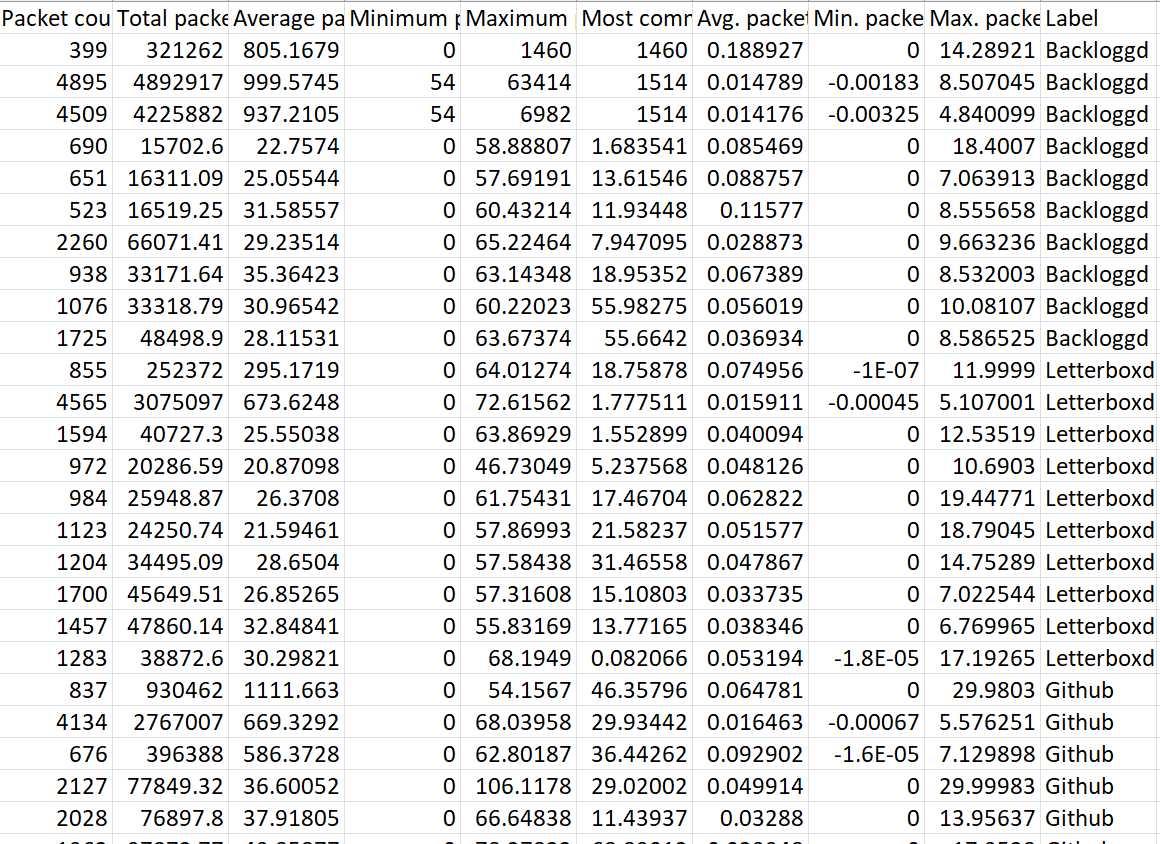
\includegraphics[width=0.99\linewidth]{data.png}
    \caption{Network traffic features extracted from each capture}
    \label{fig:1}
\end{figure}
To effectively monitor and analyze computer network traffic and classify it by website, we follow a systematic data
preparation process as shown in Fig 1.

\subsubsection{Tool Selection}
In this project, we use Wireshark [3]
(as shown in Fig 2), a highly regarded and versatile network
protocol analyzer, to collect and analyze network traffic data.
Wireshark offers a robust suite of features that allow us to
capture, decode, and inspect network traffic at the packet
level. Firstly, Wireshark provides detailed information about
individual packets, which includes information on proto
cols used, packet size, and content. This granular level of
detail is crucial for our classification tasks, allowing us to
discern specific characteristics and trends within network
traffic. Secondly, the tool supports a wide variety of protocols
and formats, making it an ideal choice for handling diverse
network environments. This flexibility ensures we can handle various types of traffic effectively. Thirdly, Wireshark’s
graphical user interface offers an intuitive way to explore
and interpret network traffic data. The interface provides features such as real-time packet capture, filtering options, and
detailed views of packet content, streamlining our analysis
process.

\subsubsection{Data Collection}
We initiate the data collection pro
cess by opening Wireshark, a network protocol analyzer,
and configuring filters to capture traffic from specific web
sites: GitHub, LetterBoxd, Backloggd, Reddit, and Weather. This
diverse selection of sites generates unique traffic patterns
representative of popular online services. We visit each web
site, navigating its pages for a minimum of one minute to
gather traffic data. This browsing session results in a single
data record containing all packets captured during that time.
We repeat this process for each of the five websites, creating
a comprehensive raw dataset. The variety of captured packets ensures a representative sample of each website’s traffic.
The data record, as illustrated in Figure 3, comprises 1423
packets, with details including Time, Source, Destination,
Protocol, and Length, providing a detailed snapshot of the
network traffic.

\subsubsection{Feature Engineering}
After collecting a sufficient number of data records, each consisting of multiple packets, we
proceed to feature engineering. The raw data cannot be directly used for training, thus we extract nine key features from each record, focusing on the dimensions of Time and
Length (as shown in Fig 4):\\\\
• \textbf{Packet Count:} This feature indicates the total number
of packets in each record, reflecting the overall communication volume. It’s a key indicator of the traffic intensity
and can reveal insights into the website’s usage patterns.\\\\
• \textbf{Total Length:} This feature represents the cumulative
size of all packets in a record, encompassing both headers
and payloads. It provides a measure of the data through
put and is crucial for understanding the traffic load and
capacity requirements.\\\\
• \textbf{Average Packet Interval:} This feature calculates the
mean time difference between consecutive packets, of inferring insights into the temporal distribution of traffic. A
higher average interval might indicate sporadic traffic,
while a lower interval suggests a steady flow.\\\\
• \textbf{Maximum Packet Interval:} This feature captures the
longest time gap between two packets in a record,helping
identify periods of inactivity or delays. This can reflect the responsiveness of the website or the nature of its
traffic.\\\\
• \textbf{Minimum Packet Interval:} This feature denotes the
shortest time gap between two packets, indicating the
speed at which data is transferred during active periods. It reflects the network’s latency and the website’s
responsiveness.\\\\
• \textbf{Average Packet Length:} This feature calculates the
mean size of all packets in a record, offering insights into
the average data volume transferred per packet. It can
indicate the nature of the website’s content (e.g., text
heavy vs. media-heavy).\\\\
• \textbf{Maximum Packet Length:} This feature indicates the
size of the largest packet in a record, reflecting the maximum data transfer capacity in a single packet. It can
reveal the presence of large files or media content.\\\\
• \textbf{Minimum Packet Length:} This feature captures the
size of the smallest packet in a record, reflecting minimal
data transfer requirements. It can indicate small, frequent
communications or requests.\\\\
• \textbf{Most Common Packet Length:} This feature represents
the size that appears most frequently among the packets,
revealing the typical packet size in the record. This can
provide insights into the website’s primary data types
and content nature.
These features provide valuable insights into the nature
of the traffic and aid in the subsequent model training phase,
allowing for the automatic classification of network traffic
by its originating website.

\subsection{Employed Method}
For our project on monitoring and analyzing network traffic,
particularly from popular internet websites, and classifying
the originating website, we employ the Random Forest algorithm [1]. This algorithm is integral to our solution due to its
flexibility, robustness, and strong performance in handling
complex classification tasks.


\subsubsection{Random Forest}
2.2.1 Random Forest. Random Forest is an ensemble learning method primarily used for classification and regression
tasks. It operates by constructing multiple decision trees during the training phase and aggregating their outputs to make
a final decision.
The process of Random Forest (as shown in Fig 5) is:\\\\
• \textbf{Building the Forest:} During training, multiple decision
trees are generated. Each tree is built from a bootstrapped
sample of the training dataset. In each tree, a subset of
features is randomly chosen to split at each node, which
helps introduce diversity among the trees.\\\\
• \textbf{Voting Mechanism:} In classification tasks, each tree votes
on the class label for a given input. The class that receives
the most votes from the trees in the forest becomes the
final prediction.\\\\
• \textbf{Robustness and Stability:} This ensemble approach makes
Random Forest resistant to overfitting, a common issue
in single decision trees, and provides a stable and reliable
model even in the face of noisy data or variations in
feature sets.
The benefits of Random Forest includes:\\\\
• \textbf{Handling Complex Features:} The task of classifying net
work traffic by its originating website involves handling
diverse and complex features,such as protocols and packet
lengths. Random Forest’s decision trees can efficiently
capture interactions between these features, producing
accurate classifications.\\\\
• \textbf{Generalization:} Due to its ensemble nature, Random For
est generalizes well to unseen data. This makes it highly
suitable for our application, where network traffic pat
terns can vary significantly between different websites
and even for the same website over time.\\\\
• \textbf{Interpretability:} While individual decision trees may be
challenging to interpret, Random Forest offers useful in
sights into feature importance. This capability is valuable
for understanding which features, such as protocol type or packet length, contribute most to distinguishing traffic
from different websites.\\\\
• \textbf{Scalability:} The Random Forest algorithm is highly scalable and can handle large datasets. This is particularly
important for our project, as network traffic data can
accumulate rapidly, necessitating a model that can efficiently handle large volumes of data.
\subsubsection{Baselines}
 We compared two baselines:
• Linear Regression [6] serves as a baseline model for
continuous numerical predictions due to its simplicity,
interpret-ability, and straightforward implementation. It
provides a linear relationship between the dependent
variable and one or more independent variables, making
it easy to understand and communicate results. The Ordinary Least Squares estimation minimizes the sum of
squared errors, offering a quick way to generate initial
predictions. Its assumptions, though restrictive, provide
a useful framework for initial model evaluation, making
it a reliable starting point for comparing more complex
models in regression tasks.
•Logistic Regression[5]is chosen as a base line model for
binary and categorical classification tasks due to its simplicity, interpretability, and effectiveness in probability
based predictions. Its logistic function directly maps features to probabilities, offering clear insight into the likelihood of a particular outcome. Maximum Likelihood
Estimation provides a robust way to fit the model to data,
and its assumptions lay the groundwork for initial model validation. This makes it a valuable baseline for comparing more complex models in classification tasks.
\section{Evaluation}
In this section, we perform an in-depth evaluation of our models and their performance on the dataset.
\subsection{Datasets}
After processing the collected data, we obtained the dataset
shown in Table 1. The train, validation, and test sets were
split with a ratio of 6:2:2.
\subsection{Evaluation Metrics}
We use two primary metrics to evaluate the models: Accuracy
and Macro F1 score. These metrics provide a comprehensive
view of performance across all classes.\\
The \textbf{Accuracy} is defined as:
\[
\text{Accuracy} = \frac{\text{True Positives + True Negatives}}{\text{Total Samples}}
\]\\
The \textbf{Precision} is defined as:
\[
\text{Precision} = \frac {\text{True Positives}}
{\text{True Positives + False Positives}}
\]
Precision indicates how many of the predicted positive
samples are actually positive.\\
The \textbf{Recall} is defined as:
\[
\text{Recall} = \frac{\text{True Positives}}
{\text{True Positives + False Negatives}}
\]
Recall reflects how many of the actual positive samples
are correctly identified as positive.
The \textbf{Macro F1 Score} is calculated by taking the harmonic
mean of precision and recall for each class, and then averaging these scores across all classes:
\[
\text{Macro F1} = \frac{1}{n}\sum_{i=1}^{n}\frac{\text{2 x Precision\_{i} x Recall\_i}}{\text{Precision\_{i} x Recall\_i}}
\]

\subsection{Evaluation Results}
The results in Table 2 show that the Random Forest model
achieves the highest accuracy (0.91) and Macro F1 score
(0.89), outperforming both Linear and Logistic Regression
models. This indicates that the Random Forest model is more
effective at capturing complex relationships in the data.
\subsection{Visualization Results}
To evaluate how each model’s predictions align with actual
values, we visualize the predictions and real values for each
model: Linear Regression (Fig 6), Logistic Regression (Fig 7),
and Random Forest (Fig 8).
The results show that the Random Forest model exhibits
the closest alignment between predictions and actual val
ues, reinforcing its superior performance observed in the
quantitative metrics.
\section{Discussion \& Future Work}

\subsection{Interpretation of Results}
Three models were tested: Linear Regression, Logistic Regression, and Random Forest. The results indicate that Random
Forest outperformed both Linear and Logistic Regression in
terms of both Accuracy and Macro F1 score. Specifically, Random Forest achieved an accuracy of 0.91 and a Macro F1 score of 0.89, compared to Logistic Regression’s accuracy of 0.83
and Macro F1 score of 0.84. This performance gap highlights
Random Forest’s ability to capture complex relationships in
the data, making it particularly suitable for network traffic
classification, where patterns can vary significantly.
The visualizations further reinforce the quantitative findings. The figures show that the Random Forest model’s predictions align closely with the actual values, providing a
visual affirmation of its superior performance.
The evaluation and comparison of these models contribute
significantly to the problem at hand: monitoring and classifying network traffic. The high accuracy and precision of
the Random Forest model allow for effective classification of
diverse traffic patterns, supporting efficient network management and optimization. This is particularly relevant for
identifying unusual or potentially harmful traffic patterns,
which is crucial for network security.
\subsection{Future Work}
Despite the strong performance of Random Forest,the project faced some challenges:\\\\
• \textbf{Dataset Size:} The relatively small dataset size might
limit the model’s ability to generalize to broader traffic
patterns. This may also impact the model’s performance
when encountering new traffic types or variations in
existing ones.\\\\
• \textbf{Handling Real-Time Data:} The current methodology
captures data from static browsing sessions, but real
world network environments often involve rapidly accumulating and dynamic traffic. This necessitates handling
real-time data streams effectively.\\\\
• \textbf{Model Complexity:} While the Random Forest model
performs well, its ensemble nature and depth can introduce interpretability challenges, making it harder to
understand which specific features drive its decisions.
To address these challenges and improve the project further, we propose the following directions:\\\\
• \textbf{Dataset Expansion:} Expanding the dataset to include
more websites and traffic records, as well as capturing
traffic patterns over longer durations, will enhance the
model’s training, making it more generalizable and robust.
Advanced Models: Exploring other machine learning
models, such as deep learning or ensemble approaches,
could further improve classification accuracy by capturing more complex traffic relationships.\\\\
• \textbf{Real-Time Processing:} Enhancing the model to handle
real-time data streams effectively will improve its practical utility in dynamic network environments. This could
involve integration with streaming analytics platforms or
developing custom solutions for real-time traffic capture
and analysis.\\\\
• \textbf{Practical Applications:} Future research should also
focus on practical applications, integrating the model
into real-world systems for network monitoring, management, and security, demonstrating its value beyond
academic contexts. This could involve collaborating with

\section{Conclusion}
In this project, we developed and evaluated a model for monitoring and classifying network traffic by its originating web
site. Using a dataset collected from diverse websites, we employed three models: Linear Regression, Logistic Regression,
and Random Forest. Through comprehensive evaluation, the
Random Forest model was found to outperform the others,
achieving the highest accuracy and Macro F1 score.
This work demonstrates the feasibility of machine learning
models, particularly Random Forest, for handling complex relationships in network traffic data. Accurate classification of
network traffic patterns contributes significantly to efficient
network management, security, and performance optimization.
The main insights include: 1) The Random Forest model’s
ensemble approach provides robustness and superior performance, particularly in handling diverse traffic patterns.
2) The project’s results indicate the importance of dataset
size and diversity in model training, highlighting the need
for expansion in future work. 3) The project’s visualizations
reveal how each model’s predictions align with actual values,
providing further insights into their effectiveness.
This project serves as a foundation for future developments in network traffic analysis, with practical implications for real-world systems and applications. By integrating
machine learning models into network monitoring, we can
enhance performance, security, and management.
% Note from the CFP that this section must include a statement about
% ethical issues; papers that do not include such a statement may be
% rejected.

%%%%%%%%%%%%%%%%%%%%%%%%%%%%%%%%%%%%%%%%%%%%%%%%%%%%%%%%%%%%%%%%%%%%%%%%%%%%
% We're in the endgame now

\bibliographystyle{ACM-Reference-Format}
\bibliography{refs}

\end{document}
